% Titre : Etude de $u_{n+1} =1 +\frac{1}{u_n}$ (Pb)
% Filiere : BCPST
% Difficulte :
% Type : DS, DM
% Categories : analyse
% Subcategories : 
% Keywords : analyse





\begin{exercice} 
Soit $\suite{u}$ la suite définie par 
$$\left\{ 
\begin{array}{ccl}
u_0&=&2\\
u_{n+1} &=&1 +\frac{1}{u_n}
\end{array}
\right.$$

\begin{enumerate}
\item Calculer $u_1$.
\item Etudiez la fonction $f: x\mapsto 1+\frac{1}{x}$. (Domaine de définition, limites et variations) 
%\item Montrer  que pour tout $n\in \N$, $1\leq u_n\leq 2$.
\item Résoudre $f(x)=x$. On note $\alpha$ l'unique solution dans $\R^*_+$. 
\item Montrer que $u_1<\alpha <2$.
\item On note $I=[1,\alpha]$ et $J=[\alpha,2]$. Montrer que $f(I)\subset J$ et $f(J)\subset I$.
\item On considère les suites $\suite{a}$ et  $\suite{b}$ définies par 
$$a_n=u_{2n} \quad b_n =u_{2n+1}.$$
Enfin on note $A$ la fonction définie pour tout $x$ par $A(x)=f\circ f(x)$.
 Montrer que $a_{n+1} =A (a_n)$. On peut montrer de manière similaire que 
 $b_{n+1} =A(b_n) $, on ne demande pas de le prouver. 
 \item Soit $F$ une fonction réelle. Soient $\cE $ et $\cF$ deux sous-ensembles de $\R$. Montrer que si $\cE\subset \cF$ alors $F(\cE)\subset F(\cF)$. En déduire que  $I$ est stable par $A$. De même, on pourrait montrer que $J$ est stable par $A$, on ne demande pas de le prouver. 
\item Montrer que pour tout $x\in D_f$, $A(x)-x =\frac{-x^2+x+1}{x+1}$ 
\item Résoudre $A(x)\geq x$ sur $]0,+\infty[$. 
\item  En déduire que $\suite{a}$ est décroissante et $\suite{b}$ est croissante. 
\item Montrer que $\suite{a}$ et $\suite{b}$ convergent, calculer leur limite. 
\item En déduire que $\suite{u}$ converge et calculer sa limite. 
\item \begin{enumerate}
\item Ecrire une fonction Python \texttt{u} qui prend en paramètre un entier $n$ et qui renvoie la valeur de $u_n$
\item Ecrire une fonction Python \texttt{limiteu} qui prend en paramètre un reel $\epsilon>0$ et  qui renvoie la valeur de du premier rang $n_0\geq 0$ tel que $|u_{n_0} -\ell|\leq \epsilon$ 
\end{enumerate}

\end{enumerate}

\end{exercice}

\begin{correction}
\begin{enumerate}
\item $u_1=\frac{3}{2}$
\item L'ensemble de définition est $\R^*$.  $f$ est dérivable sur son ensemble de définition et 
$$f'(x) =\frac{-1}{x^2}$$
On obtient le tableau de variation suivant 



\begin{tikzpicture}
   \tkzTabInit{$x$ / 1 , $f(x)$ / 2}{$-\infty$, 0, $+\infty$}
   \tkzTabVar{+/ $1$,  -D+/ $-\infty$ /$+\infty$,  -/ $1$}
\end{tikzpicture}

\item $\frac{1}{x}+1=x\equivaut x^2-1-x=0$
Dont les solutions sont $\{ \frac{1\pm\sqrt{5}}{2}\}$. L'unique solution dans $\R^+$ est $\alpha = \frac{1+\sqrt{5}}{2}$

\item $\frac{1+\sqrt{5}}{2}\leq 2 \equivaut \sqrt{5}\leq 3 \equivaut 5\leq 9$ qui est vrai. 

$u_1 \leq \frac{1+\sqrt{5}}{2} \equivaut 2\leq \sqrt{5} \equivaut 4 \leq 5$ qui est vrai. 

\item $f(\alpha) =\alpha$, $f(2) =\frac{3}{2}$. comme $f$ est décroissante sur $J$ on a bien pour tout $x\in J$ 
$f(2)\leq f(x)\leq f(\alpha)$. Donc 
$$\frac{3}{2}\leq f(x) \leq \alpha.$$ 
Comme $1\leq \frac{3}{2}$ on  a bient $f(J)\subset I$. 

Un argument similaire montre que pour tout $x\in I$ on  a:
$$\alpha =f(\alpha) \leq f(x)\leq f(1)=2$$
et ainsi $f(I)\subset J$. 
\item $\forall n\in\N$:
$$A(a_n) = f\circ f(a_n)=f\circ f (u_{2n})= f(u_{2n+1}) = u_{2n+2}=a_{n+1}$$

\item On suppose donc que $\cE\subset \cF$. Soit $y\in F(\cE)$ c'est à dire qu'il existe $x\in \cE$ tel que $f(x)=y$
Comme $\cE\subset \cF$,on a $x\in \cF$, donc $y=f(x)\in \cF$. Ainsi en tuilisant la question 5 on obtient : 
$$f\circ f(I) \subset f(J) \subset I$$

\item $A(x)=f(f(x))=f(  1+\frac{1}{x}) =1 + \frac{1}{1+\frac{1}{x}}= \frac{2x+1}{x+1} $
Donc $A(x) - x = \frac{2x+1}{x+1}  -x = \frac{2x+1-x^2 -x}{x+1} = \frac{-x^2+x+1}{x+1}$ 
\item $A(x)-x\geq 0 \equivaut \frac{-x^2+x+1}{x+1}$ dont les solutions sur $\R_+^*$ sont $S= ]0,\alpha [$. 
\item $a_0 =u_0 \in J$, comme $J$ est stable par $A$ on déduit par récurrrence que $\forall n\in \N,\, $ $a_n\in J$.
De même comme $u_1=v_1 \in I$, et $I$  est stable par $A$ on déduit que $\forall n\in \N,\,$ $b_n\in I$.
Pour tout $n\in \N$ on  a 
$$a_{n+1}-a_n= A(a_n)-a_n$$
Comme $ A(x)-x\leq 0 $ sur $J$ et $a_n\in J$, on a bien $a_{n+1}-a_{n}\leq 0$ donc $\suite{a}$ est décroissante. 

De même, pour tout $n\in \N$ on  a 
$$b_{n+1}-b_n= A(b_n)-b_n$$
Comme $ A(x)-x\geq 0 $ sur $I$ et $b_n\in I$, on a bien $b_{n+1}-b_{n}\geq 0$ donc $\suite{b}$ est croissante. 


\item Les suites $\suite{a}$ et $\suite{b}$ sont monotones et bornées. Elles sont donc convergentes d'après le théorème de la limite monotone. Notons $\ell_a$ la limite de $\suite{a}$ et $\ell_b$ la limite de $\suite{b}$ (Nous n'avons pas montré que ces suites étaient adjacentes, nous ne pouvons pas directement dire que les limites sont identiques) 

Par unicité de la limite $\lim_{n\tv infty } a_{n+1}=\ell_a$. Comme $A$ est continue sur $\R_+$ on a $\lim_{n\tv \infty} A(a_n)  = A(\ell_a)$. Ainsi $\ell_a$ vérifie $A(\ell_a) = \ell_a$. on a vu à la quetsion  9 que cette avait pour unique solution $\ell_a=\alpha= \frac{1+\sqrt{5}}{2}$. Le même argument montre que $\ell_b =\alpha$. 

\item Les deux suites extraites $u_{2n}$ et $u_{2n+1}$ convergent et ont même limite. La suite $\suite{u}$ est donc aussi convergente et a pour limite $\alpha$. 


\item 
\begin{lstlisting}
from math import *
def u(n):
  x=0
  for i in range(n):
    x=1+1/x
   return(x)

def limiteu(epsilon):
  n=0
  l=(1+sqrt(5))/2
  while abs(u(n)-l)>epsilon:
    n=n+1
  return(n)
  
def limiteu2(epsilon): #autre solution
  n=0
  l=(1+sqrt(5))/2
  u=2
  while abs(u-l)>epsilon:
    n=n+1
    u=u+1/u
  return(n)
  

def limiteab(epsilon):
  n=0
  while abs(u(2*n)-u(2*n+1))>epsilon:
    n=n+1
  return(n)
\end{lstlisting}

\end{enumerate}
\end{correction}